% !TEX root = dissertationmain.tex
\chapter{Example Application Output}

\lstdefinestyle{lineoutput}
{
    language=bash,
    backgroundcolor=\color{white},
    basicstyle=\scriptsize\color{black}\ttfamily
}


\section{Fictional Small Network Output}
\label{fictional}
\paragraph{}This output was generated by running the application in automatic, maximum verbosity, dual input with graph plotting mode. The command used to execute the application with this configuration is as follows: 
\begin{lstlisting}[language=bash]
cluster.py -s automatic -vv -p -t -N -tp ../cw.xml ../cw.nessus
\end{lstlisting}
\paragraph{}The network in which the scans were taken place is an entirely fictional and uses four machines in the scope. This scope is described below.

\begin{table}[!h]
\centering
\caption{Fictional Network Scope and Machine Descriptions}
\label{fictional_scope}
\begin{tabular}{ll}
\hline
192.168.0.1  & \begin{tabular}[c]{@{}l@{}}Windows 2008 server running Apache 2 web server with MySQL database. \\ Hosting a DNS server.\\ Domain Controller for UADTARGETNET domain \\ running Lightweight Directory Access Protocol\\ NETBIOS name: SERVER1\end{tabular} \\
\hline
192.168.0.2  & \begin{tabular}[c]{@{}l@{}}Windows 2008 server \\ running empty web server and hosting a DNS server\\ running Lightweight Directory Access Protocol\\ NETBIOS name: SERVER2\end{tabular}                                                                   \\
\hline
192.168.0.10 & \begin{tabular}[c]{@{}l@{}}Windows 7 Professional 7600 (Windows 7 Professional 6.1)\\ NETBIOS name: CLIENT1\end{tabular}                                                                                                                                   \\
\hline
192.168.0.11 & \begin{tabular}[c]{@{}l@{}}Windows 7 Professional 7600 (Windows 7 Professional 6.1)\\ NETBIOS name: CLIENT2\end{tabular}                                                                                                                                  
\end{tabular}
\end{table}


\subsection{Text Output}
\label{exampleoutput}

\lstinputlisting[style=lineoutput]{./includes/fictionaltext.txt}

\subsection{Figures}
\label{example_dual}

\paragraph{}The Figure \ref{example_twin} below shows the example graphing interface output using the configuration mentioned previously in Appendix \ref{fictional}.

\begin{figure}[!h]
\centering
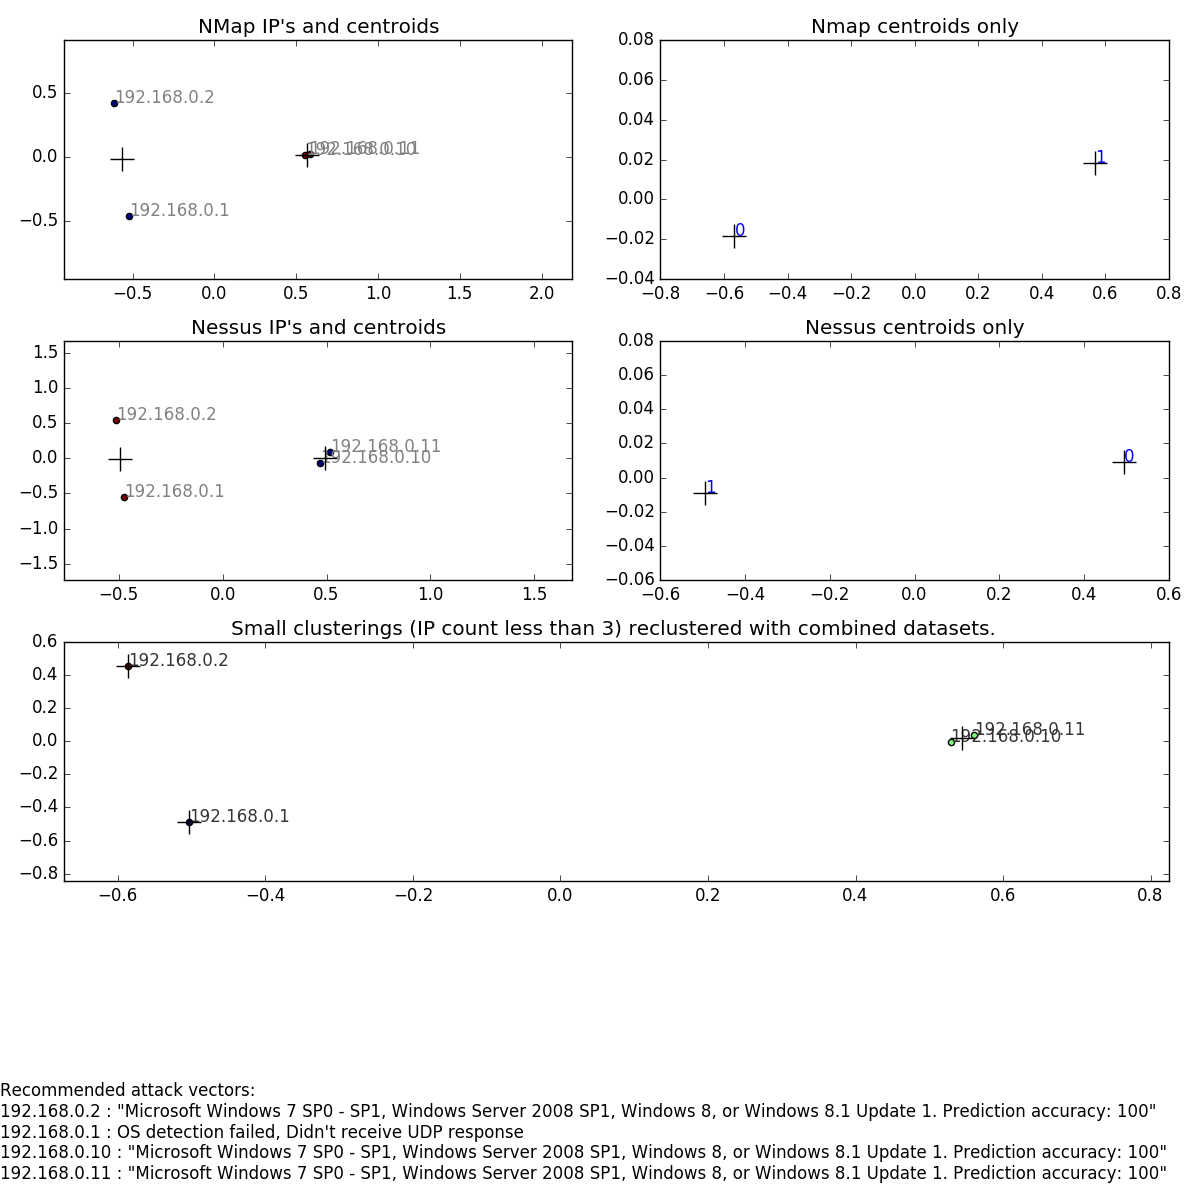
\includegraphics[width=6in]{./Figures/example_dual.png}
\caption{Example of graphing interface GUI from a fictional network to be used in conjunction with text output at \ref{exampleoutput}}
\label{example_twin}
\end{figure}


\section{Hacklab Analysis}
\label{hacklab}

\paragraph{}The following results contain outputs of the application created in this thesis when using the University Hacklab network as a dataset for scanning. The scans was obtained after permission was given on the 21st of March 2017. The IP addresses included within the scope is the entire /24 subnet with a mask of 255.255.255.0.

The nmap command used to obtain the scan was as follows:
\begin{lstlisting}[language=bash]
nmap -A -vvvv -oX test2.xml 10.0.0.0/24
\end{lstlisting}
The nessus configuration used was the default policy on an advanced scan. The target IP address configuration of 10.0.0.0/24 was used.

\subsection{Text Output}
\label{hacklabtext}
\paragraph{}The following command was issued to the application in order to achieve the output shown below. It contains the application output in very verbose dual input mode using the hacklab dataset.
\begin{lstlisting}[language=bash]
cluster.py -s automatic -vv -p -t -N -tp "../hacklab analyses/hacklab_new.xml" "../hacklab analyses/hacklab_new.nessus"
\end{lstlisting}


\lstinputlisting[style=lineoutput]{./includes/hacklabtext.txt}

\subsection{Figures}
\paragraph{}Figure \ref{split_nessus} shows the application output in standard mode using the Nessus dataset from the hacklab. The command used is as follows:
\begin{lstlisting}[language=bash]
cluster.py -s automatic -vv -p -N "../hacklab analyses/hacklab_new.nessus"
\end{lstlisting}
\begin{figure}[!h]
\centering
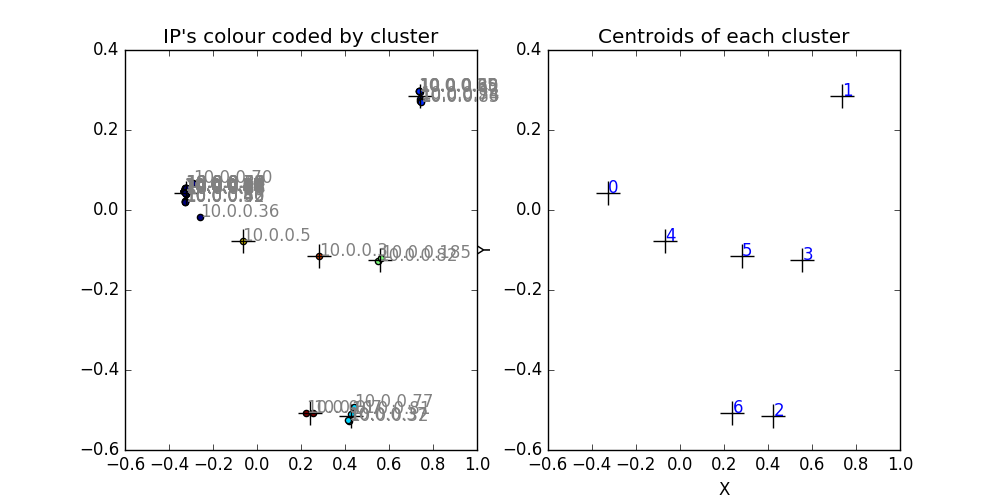
\includegraphics[width=5.5in]{./Figures/split_nessus.png}
\caption{Example graphing interface output using the the Abertay University Hacklab Nessus scan as a dataset.}
\label{split_nessus}
\end{figure}

\paragraph{}The Figure \ref{split_nmap} below shows output to that similar of the Figure \ref{split_nessus} above however this used the Nmap dataset as appose to the Nessus one used in that figure. The command used to acheive this result is as follows:
\begin{lstlisting}[language=bash]
cluster.py -s automatic -vv -p "../hacklab analyses/hacklab_new.xml"
\end{lstlisting}
\begin{figure}[!h]
\centering
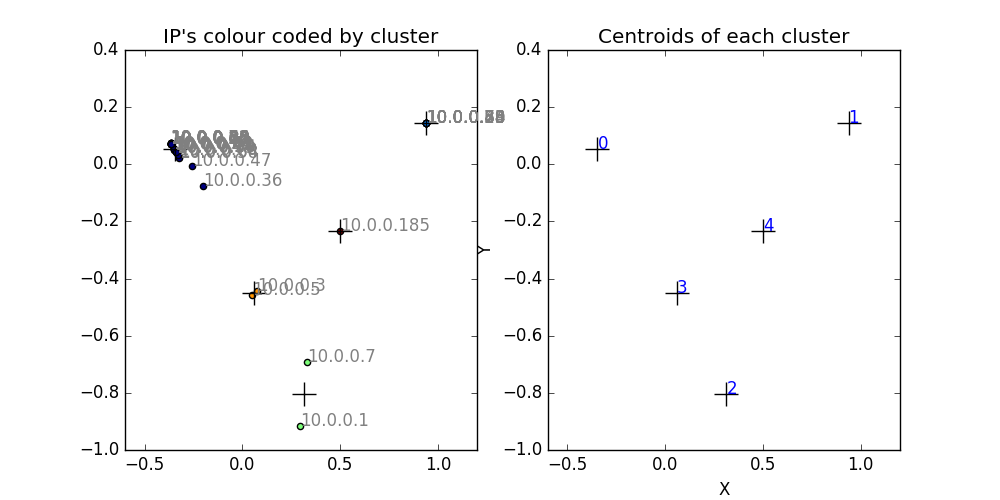
\includegraphics[width=5.5in]{./Figures/split_nmap.png}
\caption{Example graphing interface output using the the Abertay University Hacklab Nmap scan as a dataset.}
\label{split_nmap}
\end{figure}

\paragraph{} Figure \ref{dual} below shows the graphing interface opened after the completion of the clustering algorithm. This was acheived using dual mode and the command use can be found above in \ref{hacklabtext}.
\begin{figure}[!h]
\centering
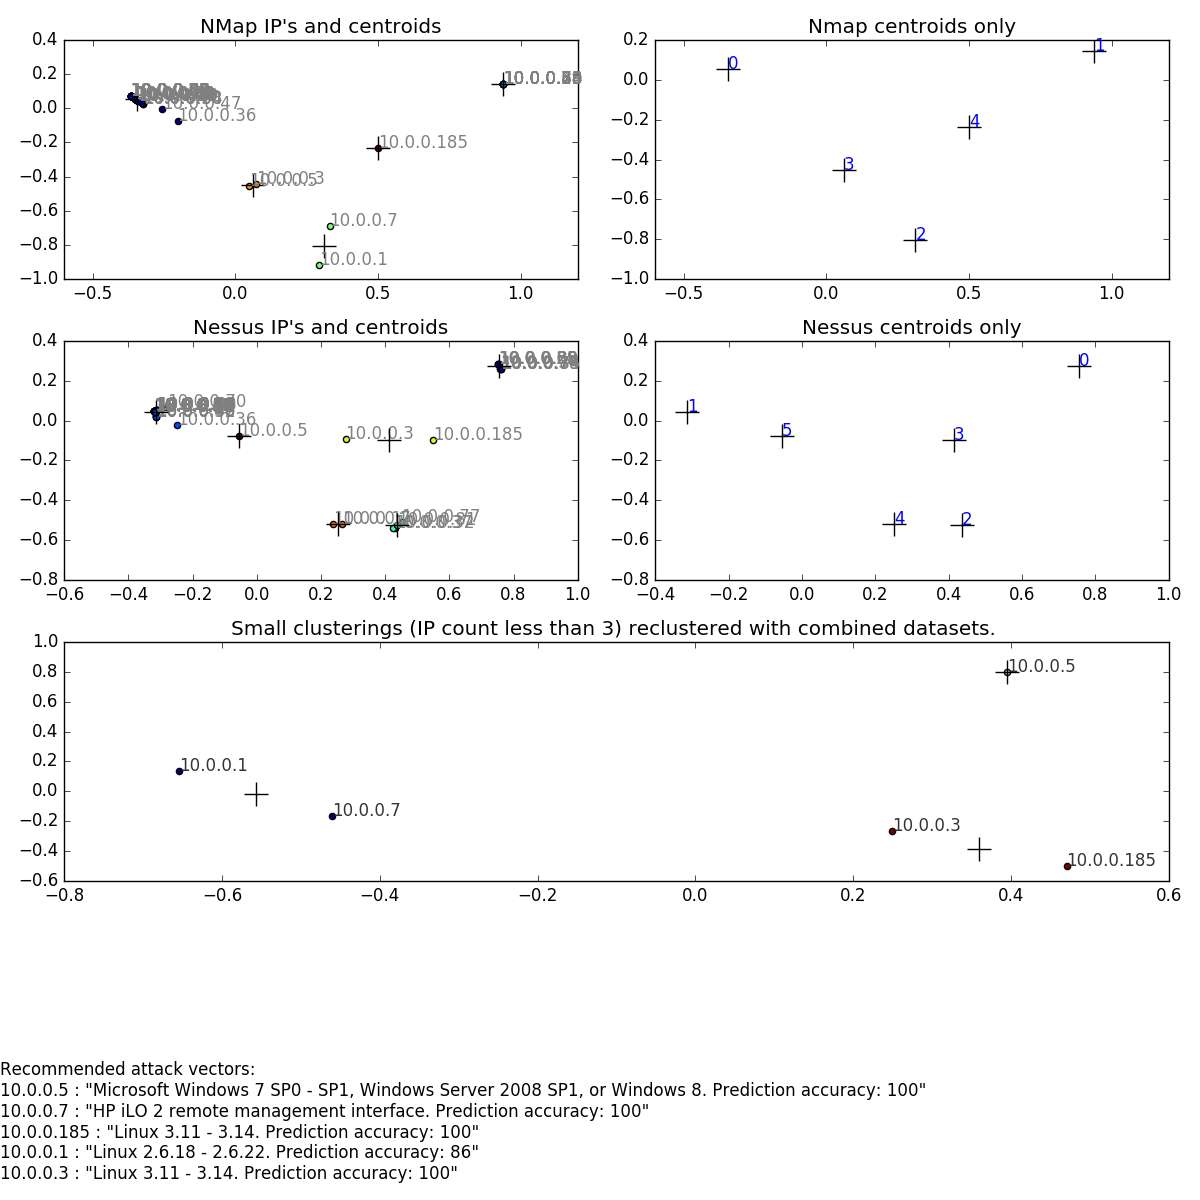
\includegraphics[width=5.5in]{./Figures/dual.png}
\caption{Example graphing interface output using both scans of Abertay University Hacklab and running the application in dual mode. }
\label{dual}
\end{figure}



